\documentclass[aps,prl,twocolumn,reprint,amsmath,amssymb]{revtex4-1}

\usepackage{epsfig,color,graphicx}
\begin{document}
\newcommand{\Ang}{\ensuremath{\mathring{\text{A}}}}
\newcommand{\ltwid}{\mathrel{\raise.3ex\hbox{$<$\kern-.75em\lower1ex\hbox{$\sim$}}}}
\newcommand{\gtwid}{\mathrel{\raise.3ex\hbox{$>$\kern-.75em\lower1ex\hbox{$\sim$}}}}
\newcommand{\ket}[1]{\ensuremath{\vert #1 \rangle}}
\newcommand{\bra}[1]{\ensuremath{\langle #1 \vert}}
\newcommand{\braket}[2]{\ensuremath{\langle #1 \vert #2 \rangle}} % bra-ket inner product
\newcommand{\ketbra}[2]{\ensuremath{\vert #1 \rangle \langle #2 \vert}} % ket-bra outer product
\newcommand{\op}[1]{\ensuremath{\hat{#1}}} % operator
%\newcommand{\sill}{\psi_\mathrm{SILL}}
\newcommand{\sill}{\psi}
\newcommand{\trace}{{\rm Tr}}
\newcommand{\ntilde}{\tilde{n}}
\newcommand{\stilde}{\tilde{s}}
\newcommand{\atilde}{\tilde{\alpha}}
\newcommand{\new}{\color{red}}
\newcommand{\old}{\color{black}}
\newcommand{\bea}{\begin{eqnarray}}
\newcommand{\eea}{\end{eqnarray}}
\newcommand{\br}{\ensuremath{\mathbf{r}}}
\def\nn{\nonumber\\}

\bibliographystyle{apsrev}

\title{Robust [LS] optimization of compact localized orbitals [in DFT]}

\author{Yifei Shi}
\author{Rustam Z. Khaliullin}
\email{rustam.khaliullin@mcgill.ca}
\affiliation{Department of Chemistry, McGill University, 801 Sherbrooke St. West, Montreal, QC H3A 0B8, Canada}

%\date{\today}

\begin{abstract}
Density functional theory based on compact localized nonorthogonal molecular orbitals is a conceptually simple method that can potentially enable low-cost linear-scaling modeling of the electronic structure of molecules and materials with finite energy gap. 
Unfortunately, its development has long been hindered because a compact representation of the electronic ground state is difficult to find in a variational optimization procedure. 
In this work, we showed that the slow and unstable optimization of compact orbitals is due to the nearly-invariant mixing of occupied orbitals that almost entirely but not fully localized within their local vector subspaces. 
%In this work, we identified the origin of the slow and unstable optimization of strictly localized orbitals and developed a simple and robust linear-scaling [optimization] procedure with a low computational overhead. 
We also proposed a simple and practical method for identifying and removing the problematic nearly-invariant modes using an approximate Hessian and, as a result, developed a robust linear-scaling optimization procedure with a low computational overhead.  
We demonstrated the new method is highly efficient yet accurate for a variety of systems ranging from molecular liquids to semi-conductors and insulators.  
%Implications.  %Although this method is not fully variational, it is still accurate enough to produce stable molecular dynamics in systems where chemical reactions happen.
\end{abstract}
\maketitle

%\emph{Introduction}

Today, Kohn-Sham (KS) density functional theory (DFT) is the most popular electronic structure method. 
The computational cost of the conventional diagonalization-based KS DFT grows cubically with the number of atoms preventing its application to large systems. 
To overcome this limitation, substantial efforts have been directed to the development of linearly-scaling (LS) DFT methods~\cite{goedecker1999linear,bowler2012methods}. 
%RZZK: perhaps it is worth mentioning that construction of the effective KS Hamiltonian is already linear, the current bottleneck is a cubically-scaling procedure for the optimization of electronic degrees of freedom.

In LS DFT methods, the delocalized eigenstates of the effective KS Hamiltonian must be replaced with an alternative set of \emph{local} electronic descriptors. 
Most LS methods explore the natural locality of the one-electron density matrix (DM)~\cite{li1993density, lee1996linear, li2003density, vandevondele2012linear, kussmann2013linear, aarons2016perspective, shao2003curvy}.  
% shao2003curvy: 10.1063/1.1558476
They include the Fermi operator expansion~\cite{goedecker1994efficient,goedecker1995tight}, divide-and-conquer~\cite{yang1991direct,yang1991local}, and direct DM optimization methods~\cite{li1993density, shao2003curvy, vandevondele2012linear}. 
However, the variational optimization of the DM is very inefficient for accurate DFT calculations which require many basis functions per atom~\cite{goedecker1999linear,vandevondele2012linear, arita2014stable, bowler2012methods, khaliullin2013efficient}.
Therefore, the application of DM-based LS methods have been mostly restricted to minimal-basis tight-binding problems~\cite{Richters2014, goringe1997tight, ratcliff2018band}. 
This issue is rectified in optimal-basis DM methods~\cite{skylaris2005introducing, nakata2015optimized, mohr2015accurate} that contract large basis sets into a small number of new localized functions and then optimize the DM in the contracted basis. 
Despite becoming the most popular LS DFT, the efficiency of optimal-basis methods is hampered by the costly optimization of both the contracted orbitals and the DM~\cite{mostofi2003preconditioned}.

From the computational point of view, a direct variation of one-electron orbitals that are strictly localized within predefined spatial regions is preferable because LS can be achieved with significantly fewer variables. %[RZZK: at least for systems with finite band gap]. 
The computational advantages of orbitals-only LS DFT are especially pronounced in accurate calculations that require many basis functions per atom. 
Strictly localized orbitals are also advantageous from the physical point of view because they provide clear, chemically meaningful, transferable description of interactions between atoms or molecules~\cite{RZZK-weitao, stoll1980use, khaliullin2007unravelling, khaliullin2008analysis}. 
%
Such orbitals are known under different names --- localized wave functions~\cite{ordejon1995linear}, nonorthogonal Wannier functions~\cite{weitao,RZZK}, absolutely localized orbitals~\cite{stoll1980use}, orbitals on compact support~\cite{RZZK}, non-orthogonal localized molecular orbital~\cite{weitao}. In this work, they will be referred to as compact localized molecular orbitals (CLMOs) to emphasize that the expansion coefficients of these orbitals in some localized basis set (e.g. numerical atomic orbitals, Gaussian orbitals, psync or RZZK-spline functions) are constrained to be precisely zero outside orbital's predefined localization region.
% RZZK: While we used ALMO -- original name given to these orbitals by Stoll et al. -- to refer to these oribtals we prefer using CLMO in this work to distinguish them from block-diagonal version of ALMO popularized in Head-Gordon et al.  
Unfortunately, the development of promising CLMO-based LS methods has been hindered~\cite{peng2013effective,tsuchida2008ab, fattebert-recent} because of inherently difficult variational optimization of CLMOs~\cite{mauri1993orbital,ordejon1995linear,goedecker1999linear, fattebert2004linear, peng2013effective, tsuchida2008ab, weitao-yang}. 
%There are also other undesirable features, manifesting depending on a particular method: multiple minima, slow convergence with large number of iterations, position of localization centers must be chosen a priori, runaway solutions, charge-conservation issues. These are not exhibited by DM-based methods (Section 3.E of Ref.~\onlinecite{goedecker1999linear}).
%
%Complete CLMO references:
%%%%%% Before Goedecker 1999
% G. Galli and M. Parrinello, Phys. Rev. Lett. 69, 3547 (1992).
% W.-L. Wang and M. Teter, Phys. Rev. B 46, 12798 (1992).
% F. Mauri, G. Galli, and R. Car, Phys. Rev. B 47, 9973 (1993).
% F. Mauri and G. Galli, Phys. Rev. B 50, 4316 (1994).
% P. Ordejon, D. Drabold, M. Grunbach, and R. Martin, Phys. Rev. B 4S, 14646 (1993).
% P. Ordejon, D. Drabold, M. Grunbach, and R. Martin, Phys. Rev. B 51, 1456 (1995).
% W. Kohn, Chem. Phys. Lett. 20S, 167 (1993).
% Further potetially important references -- must be checked:
% E. B. Stechel, A. R. Williams, and P. J. Feibelman, Phys. Rev. B 49, 10088 (1994).
% S. Goedecker and L. Colombo, Phys. Rev. Lett. 78, 122 (1994).
% T. A. Arias, M. C. Payne, and J. D. Joannopoulos, Phys. Rev. Lett. 69, 1077 (1992).
%%%%%% After Goedecker 1999 review:
%%%%%% Jean-Luc Fattebert
% fattebert2000towards https://journals.aps.org/prb/pdf/10.1103/PhysRevB.62.1713
% fattebert2002density https://onlinelibrary.wiley.com/doi/full/10.1002/jcc.10069
% fattebert2004linear https://www.sciencedirect.com/science/article/pii/S0010465504003261
% fattebert2006linear https://journals.aps.org/prb/pdf/10.1103/PhysRevB.73.115124
% oseikuffuor2014accurate https://journals.aps.org/prl/pdf/10.1103/PhysRevLett.112.046401 
%%%%%% Weitao Yang
% Yang, W., 1997, Phys. Rev. B 56, 9294.

In addition to poor convergence, a straightforward optimization of CLMOs, which cannot be constrained to stay both compact and orthogonal~\cite{stoll1980use, RZZK}, often leads to a ``collapsed'' electronic state represented by linearly dependent occupied orbitals~\cite{ordejon1995linear}. 
%
%Furthermore it was also shown in \cite{ordejon1995linear} that the straightforward LMO calculation without using a new energy functional may end up in a set of MOs that are collapsing. And the new energy functionals may lead to multiple minima \cite{kim1995total}. (Perhaps our formulation also has the multiple minima problem)
Figure~\ref{fig:det} shows that such a collapse, indicated by the vanishing determinant of the CLMO overlap matrix, is associated with 
%---caused by or causing---
the convergences problem. 

Several/Numerous efforts were made to resolve these problems. A series of work have focused on using new energy functionals~\cite{mauri1993orbital,kim1995total,ordejon1995linear} that avoid using the inverse of the CLMO overlap matrix. 
Inclusion of unoccupied orbitals~\cite{kim1995total} or extra optimization variables~\cite{burger2008linear,peng2013effective} has been proposed to mitigate convergence problems. 
% kim1995total: They do not resolve the optimization problem, they only create a method that converges to the proper minimum from ANY initial state. They judge convergence by the energy approaching a plato. They need hundreds of steps to produce a well-converged state. They are not converged even then. This can be seen from their unstable MD. How do they address the problem of multiple minima? They expand the variational space by including unoccupied orbitals and add the mu-dependent penalty designed to keep the number of electrons constant. They need to optimize mu (chemical potential) as well.
% ordejon1995linear: At each time step of the simulation, the electronic energy was minimized within a tolerance of 10$^{-8}. It is unclear what this threshold refers to. It does not seem that they use the norm of the gradient. Same problem as with kim1995total. Convergence criteria is the energy change, MD is unstable.
\new Yifei, the introduction must describe why the methods described in the reference list above were not successful in solving the convergence problem? \old Energy change as the convergence test~\cite{fattebert2000towards, kim1995total, ordejon1995linear}. Not a good convergence criterion. Does not indicate true convergence as shown in Figure~RZZK. Leads to instabilities in AIMD.
%The origins of the convergence problem have not been described. 
%Dramatically increased computational cost is one reason.

The convergence problem has been reliably solved only for weakly-interacting molecular systems. Tsuchida \emph{et al.} showed~\cite{tsuchida2007augmented,tsuchida2008ab} that CLMOs can be optimized efficiently if they are forced to be orthogonal to  a set of auxiliary tightly localized nonoverlaping orbitals, precomputed and fixed on their molecules. Similar Recently, in Ref.~\onlinecite{khaliullin2013efficient}, a block-diagonal set of orbitals is first optimized and then used to as a projector during optimization of CLMOs in the second step. These two methods have all been successful in improving the convergence by constraining the MOs to be orthogonal to some reference states, thus requiring the reference to be somewhat physically meaningful. RZZK: this only works for weakly-interacting molecular systems (the DOFs projected out already resemble the final occupied states)

Despite multiple potential advantages a reliable orbital-based LS method is still lacking for strongly interacting [nonmetallic] systems. In this work, we propose a new CLMO-based LS DFT method by identifying and projecting out the optimization directions that cause the slow convergence. The new method has the advantage that: 
\begin{itemize}
\item The energy converges fast, and works with systems where interactions are strong.
\item No ``block-diagonal reference" or ``kernel region" are needed like in \cite{tsuchida2007augmented} or \cite{khaliullin2013efficient}.
%(b) The problem of orbital collapse is avoided. (c) Exact inverse of the MO overlap matrix is used, the inversion is linear when the overlap is sparse. This prevents the error introduced by approximate inverse overlap and the problem of multiple minima. 
\item The problem of orbital collapse is avoided. 
\item Although this method is not fully variational and the energy is not the minimum of any energy functional, it still produces stable dynamics for systems involving chemical reactions. 

\end{itemize}

%fragment -> center
\label{marker:theory} 
In any CLMO method, concepts of electron \emph{localization centers} and electron \emph{localization domains} play key roles. 

In the first step, all atoms of a system, basis set orbitals localized on atoms --- in our case atomic orbitals (AOs) --- and electrons of a system are logically divided into nonoverlapping subsets called localization centers, often also referred to as fragments. For a system with clearly defined small molecules, a typical localization center includes all atoms of a single molecule and their associated basis set orbitals and electrons. For systems that cannot be partitioned into molecules --- the subject of this work --- a localization center is represented by a single atom. As a results of the partitioning, each electron acquires a localization center label. Within Kohn-Sham DFT, electrons are described by molecular orbitals (MOs) \ket{\psi_{xi}} whose indices now indicate that orbital $i$ belongs to center $x$. Throughout this work, centers are labeled with Latin letters $x,y,\ldots$ whereas with Latin letters $i,j,\ldots$ label MOs. 

In the next step, each center is assigned a predefined element-specific radius $R_c$ that is used to define neighbors for each center in an obvious way: two centers are considered neighbors if they are located within a sum of their radii. Localization domain for each center is then defined as a subset of basis set orbitals \ket{\chi_{\bar{x}\mu}} that are localized on neighbor atoms of the center. In our notation, the bar over a center index $\bar{x}$ refers to all neighbors of this center, and basis set orbitals are denoted with Greek letters $\mu,\nu,\ldots$. Thus, the basis set orbitals of a localization domain form a subspace in the one-electron Hilbert space. The following projection operator serves as the identity operator on the subspace:
%
\bea
\op{I}_{\bar{x}} = \ket{\chi_{\bar{x}\mu}} S^{\bar{x}\mu,\bar{x}\nu} \bra{ \chi_{\bar{x}\nu}},
\eea
%
where $S^{\bar{x}\mu,\bar{x}\nu}$ is a matrix element of the inverse overlap matrix $S_{\bar{x}\mu,\bar{x}\nu} = \braket{ \chi_{\bar{x}\mu}}{ \chi_{\bar{x}\nu}} $. Note that the conventional tensor notation is used to work with the nonorthogonal orbitals~\cite{head1998tensor}: covariant quantities are denoted with subscripts, contravariant quantities with superscripts, and summation is implied over the same indices. However, there is one important exception that the Einstein convention does not imply summation over centers and domains. 

%
By construction a basis set function may belong to several localization domains. Therefore, generally speaking domains overlap:
%
\begin{eqnarray}
\label{eq:span}
\hat{I} \neq \sum_{\bar{x}} \hat{I}_{\bar{x}}.
\end{eqnarray}

In the final step, the main approximation of CLMO methods is introduced. It is assumed that the electronic structure of the system can be described accurately by molecular orbitals that are completely localized within domains of their centers
%
\bea
\ket{\psi_{xi}} = \op{I}_{\bar{x}} \ket{\psi_{xi}}
\label{eq:LMO}
\eea
%
Thus this approximation imposes a blocked structure on the matrix of MO coefficients $\mathbf{T}$
%
\bea
\ket{\psi_{xi}} = \ket{\chi_{\bar{x}\mu}} {T^{\bar{x}\mu}}_{xi},
\label{eq:LMOproj}
\eea
%
opens up a possibility of performing LS calculation with MOs, and corresponds physically to electrons localized within radius $R_c$ from their centers. RZZK: comment how accurate this apprx is expected to be for finite-gap and metallic systems.


\begin{figure}
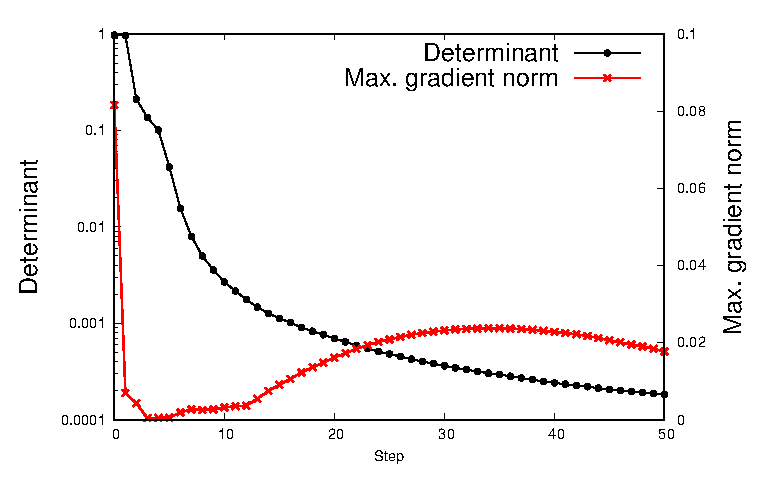
\includegraphics[width=0.5\textwidth]{det}
\caption{
The determinant of the MO overlap matrix, and maximum norm of the energy gradient. In Fig~\ref{fig:det} we show the determinant of the MO overlap matrix and the maximum norm of the energy gradient as a function of the minimization step. PBE/DZVP optimization with the preconditioned conjugate gradient algorithm. Model linear systems of four hydrogen fluoride molecules interacting through hydrogen bonds.}
\label{fig:det}
\end{figure}

In this work, we consider only spin-unpolarized orbitals evaluated at the $\Gamma$-point. The KS DFT energy functional can be written in the conventional way 
% RZZK check the equation
\bea
%E = \trace \left[ \op{R} \left(\op{t} +\op{v} + \op{H} \right) \right] + E_{\text{xc}} - \frac{1}{2}\int v_{\text{xc}}(\br) \rho(\br) d\br
E &=& 2 \trace \left[ \op{R} \op{H} \right] - \frac{1}{2} \int\int \frac{\rho(\br)\rho(\br')}{|\br-\br'|}d\br d\br' \nonumber \\
 &+& E_{\text{XC}} - \int v_{\text{XC}}(\br) \rho(\br) d\br,
\eea
%
where \op{H} is the Kohn-Sham Hamiltonian, $\rho(\br) = 2\bra{\br}\op{R}\ket{\br}$ is the electron density, and \op{R} is the projection operator onto the occupied subspace. \op{R} written to take into account the nonorthogonality of CLMOs
\bea \label{eq:dm}
\op{R} = \sum_{x,y} \ket{\psi_{xi}} \sigma^{xi,yj} \bra{\psi_{yj}},
\eea
%
where $\sigma^{xi,yj}$ is a matrix element of the inverse of the CLMO overlap matrix $\sigma_{xi,zk} = \braket{ \psi_{xi}}{ \psi_{zk}} $. %The one-electron density operator is $\op{D} = 2\op{R}$. 

A straightforward [direct?] minimization of the energy functional wrt to the variational degrees of freedom --- $\mathbf{T}$ elements --- with a preconditioned conjugate gradient algorithm (PCG) has proven a reliable low-cost method for fully delocalized orbitals ($R_c \rightarrow \infty$)~\cite{galli1992large} and completely localized orbitals ($R_c = 0$)~\cite{khaliullin2013efficient}. The PCG energy minimizer requires iterative evaluation of the energy gradient
%
\bea
{G_{\bar{x}\mu}}^{xi} \equiv \frac{\partial E}{\partial {T^{\bar{x}\mu}}_{xi}} = 4 \bra{\chi_{\bar{x}\mu}} (\op{I}-\op{R}) \op{H} \ket{\psi^{xi}}
\eea
%
and a single inversion of a preconditioner that is typically chosen as an easily-invertible approximation to the exact Hessian. We found that, for the two special cases of $R_c \rightarrow \infty$ and $R_c = 0$, the preconditioner defined on domain $\bar{x}$
%
\bea
P_{\bar{x}\mu,\bar{x}\nu} &=& 4 \bra{\chi_{\bar{x}\mu}} (\op{I}-\op{R}) \op{H}(\op{I}-\op{R}) + (\op{I}-\op{R}) \ket{\chi_{\bar{x}\nu}} 
\label{eq:hess}
\eea
%RZZK - check the prefactor. Is it 2, 4, or 8?
%
provides the same rate of convergence of the PCG algorithm as the exact Hessian but at a fraction of the inversion cost. The relation between the preconditioner in Eq.~(\ref{eq:hess}) and the exact Hessian is presented in the Supplementary Material and Ref.~\onlinecite{stoll1980use}.

In the general case of finite $R_c$, the PCG-based optmization of CLMOs could have become a low-cost linear-scaling DFT method because both \textbf{T} and \textbf{G} matrices are enforced to be sparse and the inversion of the preconditioner can be done domain-by-domain. Unfortunately, the PCG algorithm, as well as other optimization procedures based on the Newton-Raphson or DIIS-accelerated diagonalizations~\cite{stoll1980use}, suffer from the aforementioned slow convergence and orbital collapse problems. 
%
A closer inspection of the eigenvalues of the preconditioner obtained by solving the generalized eigenproblem for each domain 
%
\bea
%\mathbf{P}_{\bar{x}} \mathbf{A}_{\bar{x}} =  \mathbf{S}_{\bar{x}} \mathbf{A}_{\bar{x}} \Lambda_{\bar{x}} \\
P_{\bar{x}\mu,\bar{x}\nu} {A^{\bar{x}\nu}}_{xp} =  S_{\bar{x}\mu,\bar{x}\kappa} {A^{\bar{x}\kappa}}_{xp} \Lambda_{xp},
\label{eq:gev}
\eea
%
reveals the origin of this and other closely related previously reported problems. The eigenvalues, which approximate the energy curvature along the optimization direction \ket{d_{xp}} given by the corresponding eigenvector, ${A^{\bar{x}\nu}}_{xp} \equiv \braket{\chi^{\bar{x}\nu}}{d_{xp}}$, can be divided into three categories according to their magnitudes. Zero eigenvalues in the first category represent the optimization directions towards occupied orbitals localized completely within the same domain (Figure~\ref{fig:modes}, case A). As expected the energy is invariant along these occupied-occupied mixing modes. The second category includes large nonzero eigenvalues that represent the optimization directions towards unoccupied orbitals (Figure~\ref{fig:modes}, case B) of the domain. These two categories are the only ones present in the rapidly converging optimization of fully delocalized orbitals ($R_c \rightarrow \infty$) and completely localized orbitals ($R_c = 0$). The eigenvalues classified as the third category are extremely small but nonzero. They appear only for finite $R_c$ when orbitals on different domains share basis set functions. 
The optimization along these low-curvature nearly-invariant directions is difficult to converge because various analytical approximations (e.g. approximate Hessian, quadratic linear search) and numerical noise (e.g. finite DFT grids) make calculations too imprecise. Thus the presence of the low-curvature modes represents the major barrier to the practical use of promising orbital-based LS DFT methods. Fig~\ref{sfig:hesseig} int the supplementary material shows an example of such small eigenvalues.

\begin{figure*}
\centering
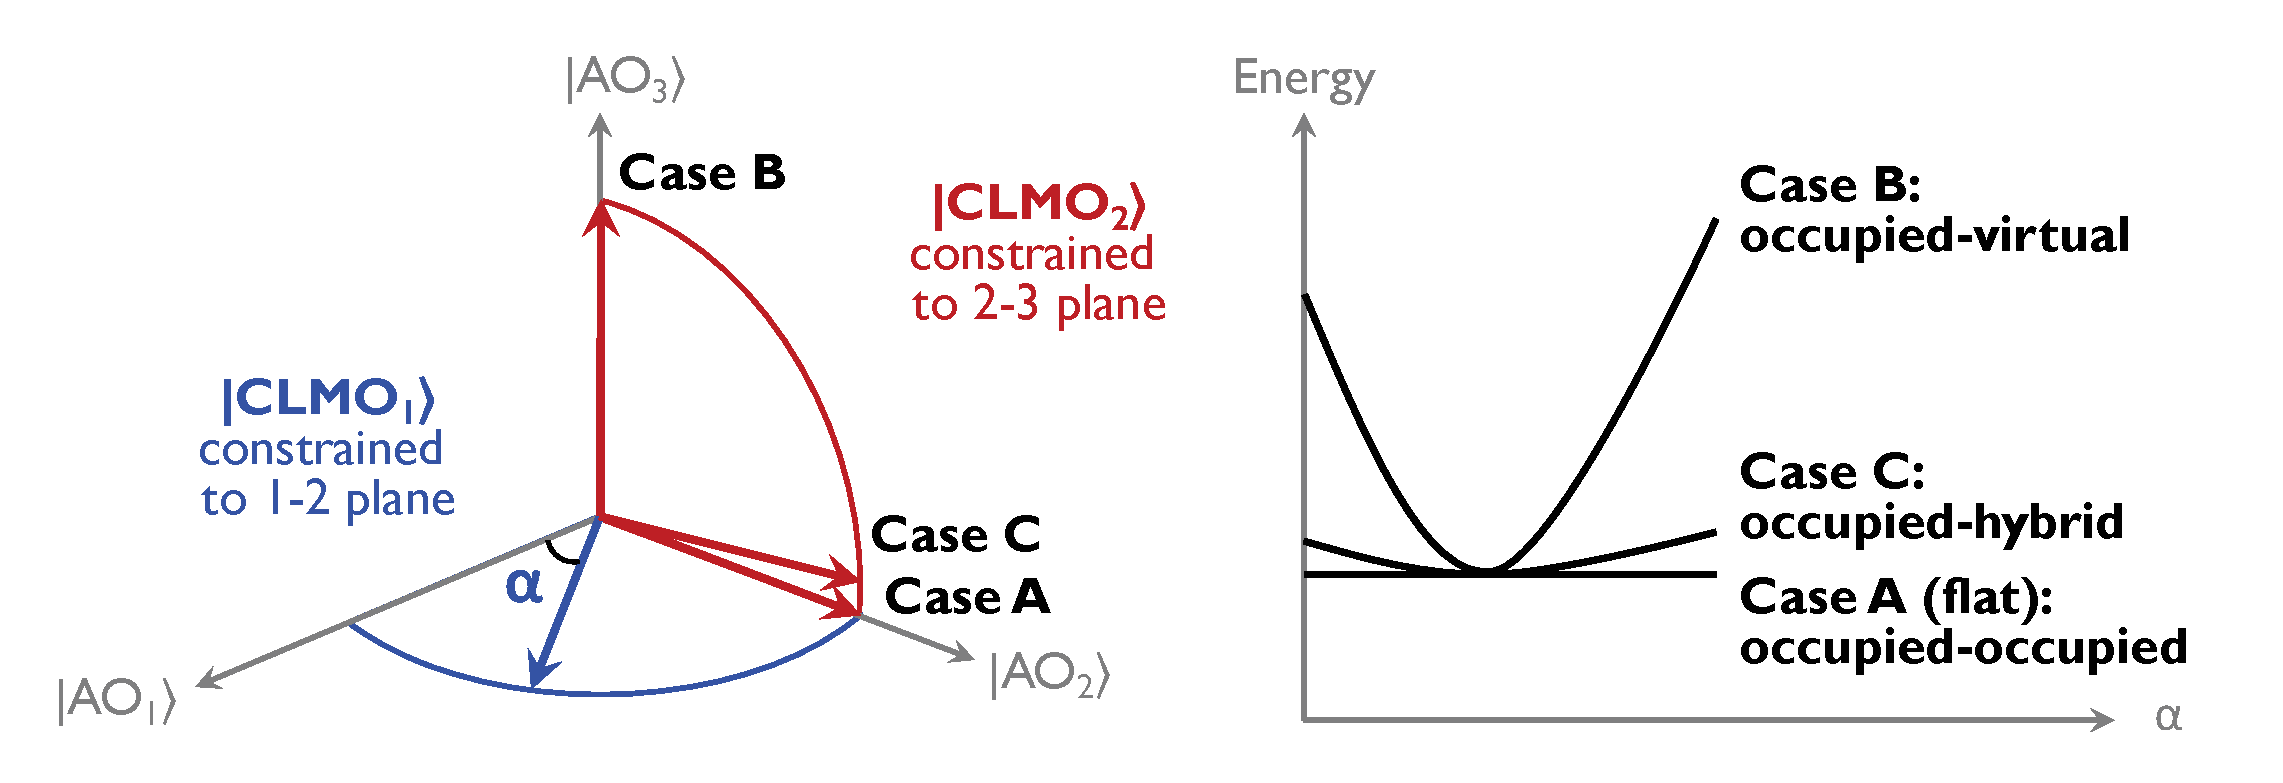
\includegraphics[width=0.8\textwidth]{modes}
\caption{Illustration of the origin of low-curvature modes in a model vector space spanned by three basis set functions \ket{\text{AO}_1}, \ket{\text{AO}_2}, \ket{\text{AO}_3}. The left panel shows \ket{\text{CLMO}_1} (blue) confined to its domain spanned by \ket{\text{AO}_1} and \ket{\text{AO}_2} as well as \ket{\text{CLMO}_2}  (red, three cases) confined to its domain spanned by \ket{\text{AO}_2} and \ket{\text{AO}_3}. The right panel shows the behavior of the energy as a function of the position of \ket{\text{CLMO}_1} --- angle $\alpha$ --- for three typical cases. Case C shows that the low-curvature modes arise when \ket{\text{CLMO}_2}  lies almost entirely in the domain of \ket{\text{CLMO}_1}.}
\label{fig:modes}
\end{figure*}


\label{marker:nature} 

What is the physical origin of the low-curvature optimization modes? 
It has been suggested previously~\cite{goedecker1999linear} that the sluggish optimization in orbital-based LS DFT is due to the inexact invariance of the energy wrt the mixing of occupied orbitals. 
Although this might indeed present a problem for a series of approximate functionals~\cite{Galli} the density matrix used in this work is constructed with the inverse of the overlap matrix and, therefore, is properly idempotent and exactly invariant to the mixing among occupied states. 
We instead suggest that the low-curvature modes correspond to the ``almost'' (RZZK: is it better to call them mixed modes?) occupied directions illustrated in Figure~\ref{fig:modes}, case C. 
This hypothesis can be verified by calculating the norm of the component of the small-curvature directions \ket{d_{\bar{x}p}} in the unoccupied space:

%Yifei: in reality, \op{I}_{\bar{x}} is not used but instead an operator to pick out only indices belonging to domain x
%
\bea
\label{eq:residue}
\Delta_{\bar{x}p} = \bra{d_{\bar{x}p}} \op{I}_{\bar{x}} - \op{R}_{\bar{x}} \ket{d_{\bar{x}p}} 
\eea
%
where $\op{R}_{\bar{x}}$ is defined, somewhat arbitrarily, as
% RZZK: re-write the equations to explain what is really done.
%RZK: the projector must be redefined to include only orbitals that are significantly present on \bar{x}
\bea
{R}_{\bar{x}} &=& \sum_{y,z} \op{I}_{\bar{x}} \ket{\psi_{yi}} \sigma_{\bar{x}}^{yi,zj} \bra{\psi_{zj}} \op{I}_{\bar{x}}
%R^{\bar{x}\mu,\bar{x}\nu} &\equiv& \bra{\chi^{\bar{x}\mu}} \op{R}_{\bar{x}} \ket{\chi^{\bar{x}\nu}} \\
\label{eq:C}
\eea
%
and $\sigma_{\bar{x}}$ is the overlap matrix of $\bar{x}$-projected orbitals
%
\bea
\left(\sigma_{\bar{x}}\right)_{yi,zj} = \bra{\psi_{yi}} \op{I}_{\bar{x}} \ket{\psi_{zj}}
\eea
%
Our hypothesis implies that $\Delta$ should be small for all small-curvature eigenvectors. 
Figure~\ref{fig:projection} shows that indeed the small-curvature modes indeed lie within the occupied space for a variety of materials. See supplementary material for more details. 
It is also interesting to note that the ``unoccupied'' fraction of the low-curvature modes increases with increasing strength of intercenter electron delocalization, that is, with the degree of covalency of interatomic bonding. %RZZK: detailed expalnation why this is so.
Thus the optimization along the low-curvature modes mixes orbitals that are almost completely but not fully occupied (RZZK: mixed is a better definition). Unsurprisingly, such varying orbitals along these directions often leads to their collapse. 

The proposed explanation of the nature of the low-curvature modes is consistent with the fact that, for molecular partitioning, their number is equal to the sum of occupied orbitals on the neighbor centers. It also explains why the two-step procedure of Ref.~\onlinecite{khaliullin2013efficient} works so well for molecular systems. %RZZK: In the two-step procedure block-diagonal (i.e. $R_c=0$) orbitals are optimized first and then the trial orbitals are optimized with the block-diagonal CLMOs projected out, Block-diagonal ALMOs are good “shadows” because they are already close to the final delocalized orbitals. 

\begin{figure}
\centering
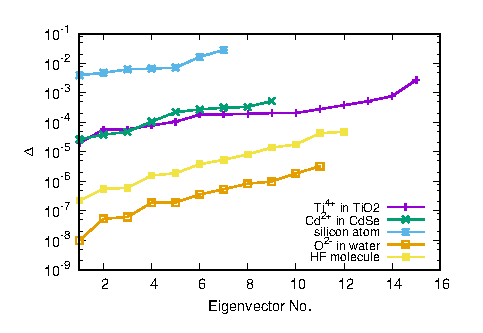
\includegraphics[width=0.5\textwidth]{residue}
\caption{
The norm of the projection of the small-curvature modes on the unoccupied subspace of a domain. 
The BLYP/TZV2P level of theory is used for water and PBE/DZVP in all other tests. 
Preconditioner eigenvectors with the eigenvalues smaller than 0.02~a.u. are chosen as small-curvature modes. 
The following localization ceneters are considered: Ti$^{4+}$ ions in the TiO$_2$ rutile lattice, Cd$^{2+}$ ions in the CdSe Wurtzite lattice, Si atom in the diamond silicon lattice, O$^{2-}$ in a water tetramer system, hydrogen fluoride molecule in a linear tetramer system.}
%Yifei: Localization centers are listed, domains also include neiboring atoms as well, which are for each system considered: Ti$^{4+}$ and 4 O$^{2-}$, Cd$^{2+}$ and 3 Se$^{2-}$, 5 Si atoms, two water molecules, 3 HF molecules
%RZK: Y axis labels: $\Delta$ instead of "Residue". X axis label "Eigenvector No.". X axis starts with 1. The legend should mirror the caption: "Ti$^{4+}$ in TiO$_2$" and so on. Include the same water system with atomic partitioning. Consider plotting more modes, including what we call category-2 modes.
\label{fig:projection}
\end{figure}

%The intuition from Eq~(\ref{eq:baddir}) implies that for each fragment $x$, each neighboring MO $|\psi_{yj}\rangle$ that only have a small portion outside of $x$ would contribute one problematic direction $P^x | \psi_{yj}\rangle$. And $Q^x$ should be a projector that removes all these directions, we assume MO $i$ on fragment $y$ that only have very small part outside of $x$, it will be denoted $xyi$, and the common AOs of $x$ and $y$ fragments are denoted $xy\mu$, then $Q^x$ can be approximated as:
%%
%\bea
%(Q^x)^{x\mu,x\nu} \approx S^{x\mu,x\nu} - T^{xy\mu}_{yi} (\sigma^{-1})^{xyi,xzj} T^{xz\mu}_{zj}
%\label{eq:approxq}
%\eea

%In some extreme cases, there might be not sufficient DOFs within a domain to . 
Figure~\ref{fig:convergence} shows that the two-step procedure is not efficient for a system of strongly interacting atoms, namely, silicon atoms in the cubic diamond phase. This is because the block-diagonal projector $\op{R}^0$ does not adequately represents the low-curvature modes. [In fact, it is difficult to construct a trial CLMO that is both simple and .] Therefore, instead of performing the two-step procedure we propose to solve the problem of sluggish convergence by detecting the low-curvature modes directly by diagonalizing the approximate Hessian in Eq.~\ref{eq:hess} and avoiding the optimization along these modes altogether. Although this procedure does not produce fully optimized orbitals they are still expected to provide accurate representation of the ground state. This is because low-curvature directions are also ``shallow'' directions, that is, they do not produce a significant variational decrease in energy. To filter out low-curvature modes we construct a projector
\bea
%L^{\bar{x}\mu,\bar{x}\nu} &=& {A^{\bar{x}\mu}}_{xp} \Theta_{xp} {A^{\bar{x}\nu}}_{xp} \\
\op{Q}_{\bar{x}} &=& \ket{d_{\bar{x}p}} \Theta_{\bar{x}p} \bra{d_{\bar{x}p}},
\eea
%
where $\Theta$ is zero if the corresponding mode is a low-curvature mode and one otherwise. This projector is applied to the gradient and preconditioner
%
\bea
%{Q_{\bar{x}\mu}}^{\bar{x}\lambda} &=& \bra{\chi_{\bar{x}\mu}} \op{I}_{\bar{x}} - \op{W}_{\bar{x}} \ket{\chi^{\bar{x}\lambda}} \\
\tilde{G}{_{\bar{x}\mu}}^{xi} &=& {Q_{\bar{x}\mu}}^{\bar{x}\lambda} {G_{\bar{x}\lambda}}^{xi} \\
%
\tilde{P}_{\bar{x}\mu,\bar{x}\nu} &=& {Q_{\bar{x}\mu}}^{\bar{x}\lambda} {P}_{\bar{x}\lambda,\bar{x}\gamma} {Q^{\bar{x}\gamma}}_{\bar{x}\nu}
\eea
%
and the projected gradient and preconditioner are used in the PCG algorithm. 

As a result, the optimization procedure neglects low-curvature modes and the hopefully small energy changes associated with them. Figure~\ref{fig:convergence} shows that the new optimization procedure becomes robust for a challenging case of atomic partitioning of the hexagonal CdSe lattice (Figure~\ref{fig:convergence}). At the same time, the final energy is close to the CLMOs energy obtained variationally using the two-step method of Ref.~\cite{khaliullin2013efficient}. 

\begin{figure}
\centering
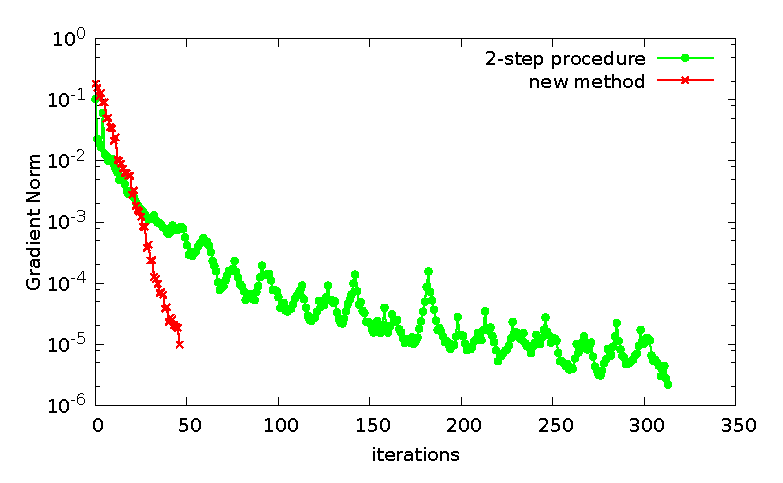
\includegraphics[width=0.5\textwidth]{convergence}
\caption{The maximun norm of the energy gradient for the PBE/DZVP-MOLOPT basis optimization of the CLMOs for Cdse lattice. $R_c = 3.5$~{\AA}. Modes with the preconditioner eigenvalues lower than 0.05~a.u. are removed from the optimization. The difference in the ground state energy for the two methods is 0.03 kJ/mol per Cd atom.}

%RZK: Legend: replace "2-step procedure" with "Block-diagonal projector"; replace "new method" with "Low-curvature projector" Axis: replace "Gradient Norm" with "Max. gradient norm"; replace "iterations" with "Iteration". Explain legend in the caption. Are we sufficiently well converged to report the difference in energy reliably? 
\label{fig:convergence}
\end{figure}


STOPPED HERE: 

Describe how low-curvature modes are selected.

Show that the procedure is robust, results are accurate, computations are LS and low-cost. Compare to DM methods?

Discuss advantages and weaknesses of the new method

while giving up a strict energy functional: the final energy may depend on the optimization path. However, we demonstrate that the energy is still accurate enough and can produce stable molecular dynamics nonetheless.
We also note that the preconditioner does not need to be calculated for each step, improving the efficiency of the optimization. 

As stated before, the filterd directions should be primarily occupied-occupied mixing, so that physically meaning full directions are not neglected and the final state is close to the true ground state. 

%To see how similar $C$ and $W$ really are, we calculate the principle angles between them\cite{hotelling1936relations}, characterizes the difference between the two subspaces. When all the principle angles are zero, the two subspaces are exactly the same. They can be calculated from the single value decomposition of the product of the two projectors: 
%\bea
%C\cdot W = U\cdot \Sigma \cdot V 
%\eea
%where $U$ is a $N\times r$ dimensional matrix and $V$ $r\times N$ dimensional. The eigenvalues corresponds to the cosine of the principle values. 
%We note that although $C$ and $W$ are very close, the more intuitive and easier-to-calculate $C$ cannot be used to eliminate the problematic directions completely and thus is not used to optimize LMOs.


\label{marker:results}

The procedure for selecting and projecting out the low-curvature modes is implemented in the CP2K package\cite{cp2kgeneral}. which uses the mixed Gaussian and plane wave method\cite{vandevondele2005quickstep}, and is an ideal platform for LS method. The optimization scheme is applied to systems with small band gap which are typically difficult for LS methods. The inversion of MO overlap matrix is carried out using Hotelling method \cite{hotelling1943some} which is linear scaling when the overlap matrix is sparse. Fig~\ref{fig:accuracy} shows the energy as a function of $R_c$ for several different systems: (a) CdSe on hexagonal wurtzite lattice with 768 atoms. (b) 64 water molecules, where each fragment is an atoms, and there are strong interaction and significant electron delocalization between fragments. (c) dimond Si of 512 atoms. We note that upon applying the filter $Q^x$ on the gradient, the final energy is no longer fully variational: the gradient is only zero in diretions that significantly change the energy. It also implies that the energy will depend on the optimization path. However, it is clear from Fig~\ref{fig:accuracy} that the energy converges to the DFT value as a function of cutoff, and the error mentioned is neglectable. 

\begin{figure}
\centering
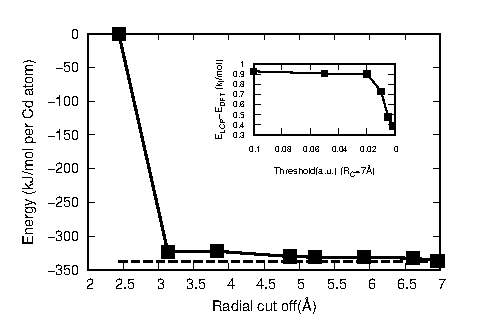
\includegraphics[width=0.35\textwidth]{CdSe_conv}
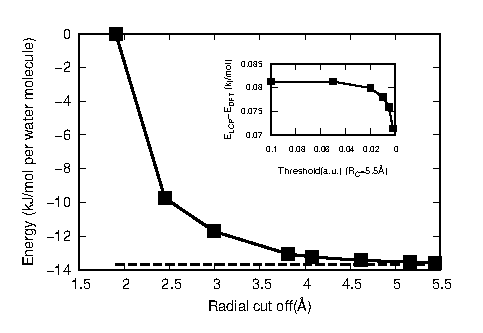
\includegraphics[width=0.35\textwidth]{H2O_conv}
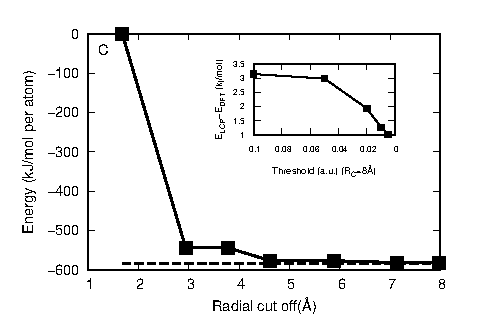
\includegraphics[width=0.35\textwidth]{Si_conv}
\caption{Energy from the low-curavture projector and the dependence on the localization radii $R_c$ for (a) PBE/DZVP calculation for CdSe in a hexagonal wurtzite lattice, (b) BLYP/TZV2P calculation for liquid water with atomic partitioning, (c) PBE/DZVP calculation for cubic diamond phase of silicon. The convergence criteria is $\vert\vert G\vert\vert_{\text{max}} < 10^{-5}$. Zero energy is set at the block-diagonal reference. Dashed line shows the reference energy of conventional DFT calculation(E$_{\text{DFT}}$) without localizatioin constrains(R$_c\rightarrow \infty$). \\
Inset: Low-curvature-projector(E$_{\text{LCP}}$) energy dependence on the low-curvature threshold at a fixed $R_c$, the zero energy is set to be E$_{\text{DFT}}$. }
%Yifei: Used kJ/mol for most energy units. I also convered length unit vdW radii to angstrom by looking up the data base. However the original cutoff is different for different atoms, which I didn't mention for simplicity.
\label{fig:accuracy}
\end{figure}

\label{marker:performance}To test the computational efficiency of the newly designed method, we compared its performance to the orbital transformation (OT) optimizer \cite{weber2008direct,vandevondele2003efficient} --- a well-optimized low-prefactor cubic scaling DFT method for conventional fully delocalized orbitals. The calculation is done for hexagonal CdSe of different system sizes. $R_c$ is set to 3.5~{\AA}, which is large enough to accurately describe the electronic structure of the system (Figure~\ref{fig:accuracy}). Figure~\ref{fig:scaling} demonstrates that our method is asymptotically LS. The LS regime is achieved when the MO overlap matrix and its inverse are sufficiently sparse. For a dense system like CdSe it takes on the order of $\sim$3000 atoms. RZZK: should we compare to a typical DM method?

\begin{figure}
\centering
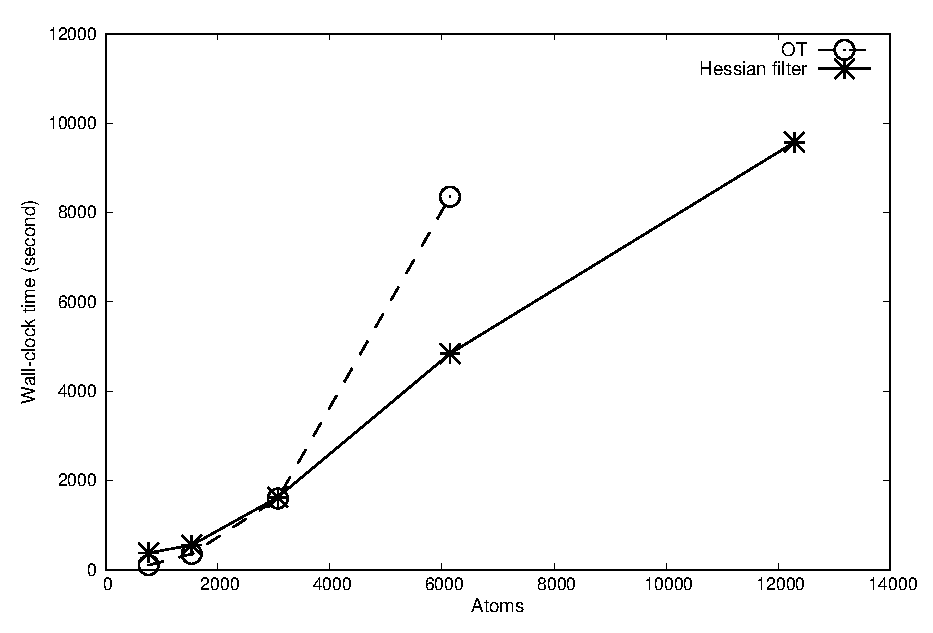
\includegraphics[width=0.45\textwidth]{timing}
\caption{CLMO optimization timing benchmark for CdSe. The PBE/DZVP-MOLOPT basis calculation with $R_c=3.5$~{\AA} is done on 256 cores.}
\label{fig:scaling}
\end{figure}


\label{marker:moldyn} The accuracy of force calculation is crucial to a stable molecular dynamics (MD) simulation. A preliminary test of our method is done on a system of 62 water molecules with 2 H$^+$ atoms. The 2 protons will hop around through OH covalent bond breaking and reforming. Here each atom is a localization center, resulting strong covalent interaction and bond breaking between fragments. We show in Fig~\ref{fig:md} the conserved quantity and the potential energy in a MD run of 2 picoseconds. We note that the Hellmann--Feynman theorem\cite{feynman1939forces} is used for the calculation of the force, this is in general only true when the energy is full variational, which is not true in our case. This is the reason of noise of constant quantity in the simulation. While this is just a preliminary test of the method and force evaluation is not the focus of this paper, we believe modifications to the MD algorithm(for example, the modified Langevin integrator method in Ref~\onlinecite{scheiber2018communication}) could further stablize the calculation.

\begin{figure}
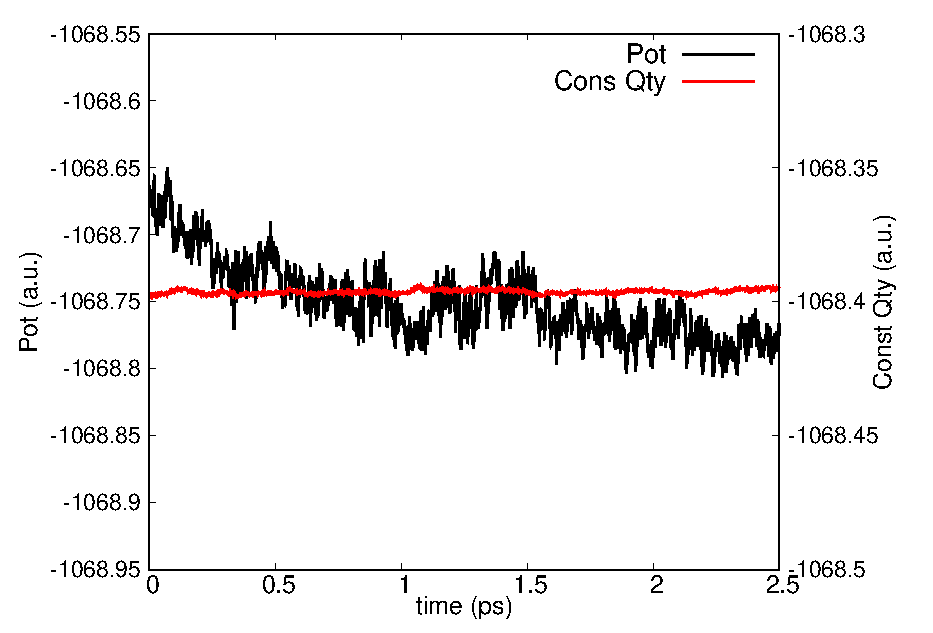
\includegraphics[width=0.45\textwidth]{const.eps}
\caption{The potential energy (Pot) and constant quantity (Const Qty) during a MD simulation using low-curvature-projector method with NVT ensemble. The temperature of simulations was set to 298~K and was controlled by a canonical velocity re-scaling thermostat\cite{bussi2007canonical} with the coupling time constant set to 50 fs.}
\label{fig:md}
\end{figure}

To further demonstrate the accuracy of the energy calculation, we perform Monte Carlo (MC) simulation of a defected dimond silicon lattice, where 2 neighboring silicon atoms are replaced by 2 carbon atoms. The resulting silicon-silicon radial distribution function (RDF) is shown in Fig~\ref{fig:mc}. For comparison we also show the RDF calculated from molecular dynamics simulation using OT. 

\begin{figure}
\centering
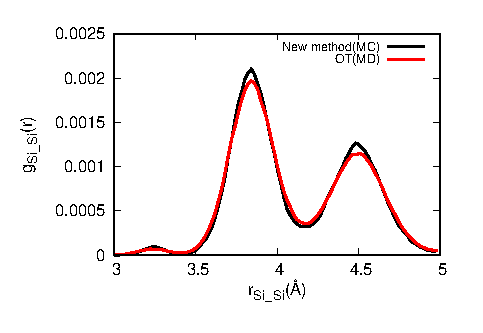
\includegraphics[width=0.45\textwidth]{rdf_si}
\caption{Radial distribution calculated with MC using the new method, and OT with molecular dynamics. The temperature is set at 500K, the systems includes 62 silicon atoms and 2 carbon atoms, periodic boundary condition is used.}
\label{fig:mc}
\end{figure}

\label{marker:conclusion} We develop a new DFT method based on LMOs. The notorious convergence problem is avoided by identifying the small but none-zero eigenvalues of the Hessian. These directions are projected out from the gradient and the preconditioner, and the remaining gradient shows fast convergence with PCG. This projection can be understood as a relaxed orthogonality constrain for the LMOs. This method works even when the interaction and covalency between fragments are strong. We demonstrate the accuracy and efficiency of the method on systems like dimond silicon, CdSe. We also show a MD simulation in liquid water containing protons, and show that it can deal with systems where chemical reactions happen.

While many previous works~\cite{RZZK} dealt with weakly-interacting fragments (e.g. molecules) the approach here represents the ultimate atomic partitioning scheme. This partitioning allows to study chemical processes in the course of simulations without resorting to complex and unreliable schemes that redefine molecular fragments on-the-fly.

Add to discussion: One weakness of defining CLMO domains \emph{a priori} in this way is that at least rough idea about the electron distribution in a system is required to assign electrons to localization centers and domains. Such a procedure is, of course, not applicable to systems in which the exact bonding properties are unknown.

RZZK: The physical meaning of Eq~\ref{eq:approxq} is a modified orthogonality constrain for LMOs. Orthognality and locality has generally been considered as competing properties: strict orthogonality leads to decaying tails, and for LMOs no orthogonality constrains are imposed except for MOs within a fragment. However, this causes the convergence problem previously mentioned: LMOs without orthogonality tends to collapse. Although global orthogonality cannot be achieved, we suggest a local orthogonality constrain, that the projection of MOs onto each fragment $x$ should be orthogonal. Unlike the case for none-local MOs, not every physical state can be transformed into such state.

\section{Acknowledgments} The research was funded by the Natural Sciences and Engineering Research Council of Canada through the Discovery Grant. The authors are grateful to Compute Canada and McGill HPC Centre for computer time.

\bibliography{negref}

\section{Supplemental Material}

\setcounter{equation}{0}
\setcounter{figure}{0}

\renewcommand{\theequation}{S\arabic{equation}}
\renewcommand{\thefigure}{S\arabic{figure}}

\subsection{Details of matrix equations}
Matrix equations clarify more compact operator expression used in the main text. 

%The energy:
%\bea
%E[\{\psi_i\}] &=& 2\sum_{i,j} (\sigma^{-1})_{ij}\int \psi_i (\br) h(\br) \psi_j(\br) d\br \nonumber \\
%&+& \frac{1}{2} \int \int \frac{\rho(\br)\rho(\br')}{|\br-\br'|}d\br d\br' + E_{XC}[\rho] 
%%\\
%%&+& 2\sum_{i,j} (\sigma^{-1})_{i,j}\int \psi_i(\br) \psi_j(\br) d\br \nonumber
%\eea
%%
%where $h(\br)$ is the combine kinetic and nuclear-electron attraction energy operator
%%
%\bea
%h(\br) \equiv -\frac{1}{2}\nabla^2 + v_{\text{ext}}({\br}),
%\eea
%%
%$\rho(\br)$ is the electron density
%%
%\bea
%\rho(\br) \equiv 2 \sum_{i,j} (\sigma^{-1})_{ij} \psi_i(\br) \psi_j(\br) ,
%\eea
%%
%and $\sigma$ is the CO overlap matrix
%%
%\bea
%\sigma_ij \equiv  \int \psi_i (\br) \psi_j(\br) d\br .
%\eea
%%

Contravariant density matrix:
%
\bea
\mathbf{R} = \mathbf{T} \sigma^{-1} \mathbf{T}^{\dagger}
\sigma = \mathbf{T}^{\dagger} \mathbf{S} \mathbf{T}
\eea
%
or, using the element by element notation,
%
\bea
R^{w\mu,z\nu} = \sum_{x,y}{T^{\overline{wx}\mu}}_{xi} \sigma^{xi,yj} {T^{\overline{zy}\nu}}_{yj}
\eea

The gradient for domain $\bar{x}$
%
\bea
\mathbf{G}_{\bar{x}x} = 4 \left[(\mathbf{I}-\mathbf{SR}) \mathbf{H} \mathbf{T}\sigma^{-1} \right]_{\bar{x}x}
\eea
%
or
%
\bea
{G_{\bar{x}\mu}}^{xi} = 4 \left[(\mathbf{I}-\mathbf{SR}) \mathbf{H} \mathbf{T}\sigma^{-1}\right]{_{\bar{x}\mu}}^{xi}
\eea
%

The preconditioner for domain $\bar{x}$ 

%
\small {
\bea
P_{\bar{x}\bar{x}} &=& s_x \left[(\mathbf{I}-\mathbf{SR}) \mathbf{H}(\mathbf{I}-\mathbf{RS}) + (\mathbf{I}-\mathbf{SRS})\right]_{\bar{x}\bar{x}} 
\eea 
%
\bea
P_{\bar{x}\mu,\bar{x}\nu} &=& s_x \left[(\mathbf{I}-\mathbf{SR}) \mathbf{H}(\mathbf{I}-\mathbf{RS}) + (\mathbf{I}-\mathbf{SRS})\right]_{\bar{x}\mu,\bar{x}\nu} 
\eea 

$\bar{x}$-coefficients of the $y$-centered orbitals projected onto $\bar{x}$-space are determined by
%
\bea
\op{I}_{\bar{x}} \ket{\psi_{yi}}  &=& \ket{\chi_{\bar{x}\mu}} S^{\bar{x}\mu,\bar{x}\nu} \braket{ \chi_{\bar{x}\nu}}{ \chi_{\bar{y}\lambda}}\, {T^{\bar{y}\lambda}}_{yi} = \nonumber \\
 &=& \ket{\chi_{\bar{x}\mu}} \left[ S^{\bar{x}\mu,\bar{x}\nu} S_{\bar{x}\nu,\bar{y}\lambda} {T^{\bar{y}\lambda}}_{yi} \right]
\eea 
}
%
Note that coefficients outside $\bar{x}$ may be nonzero but we do not need them.

\subsection{Generalized eigenvalues of Hessian, and physical meaning of low-curvature-projector}

Here we further illustrate the origin of slow converging modes by looking at the (generalized) eigenvalues of the Hessian in the calculation of a realistic system. Fig~\ref{sfig:hesseig} shows the cases of (a)completely delocalied calculation, where the eigenvalues are either 0(corresponding to a occupied-occupied mixing) or significanly large(occupied-virtual mixing). (b) Straight forward CLMO calculation, where the eigenvalue spectrum is continuous and intermediate modes exsit. (c) Low-curvature-projector method, where the small and large eigenvalues are again seperated.

\begin{figure}
\centering
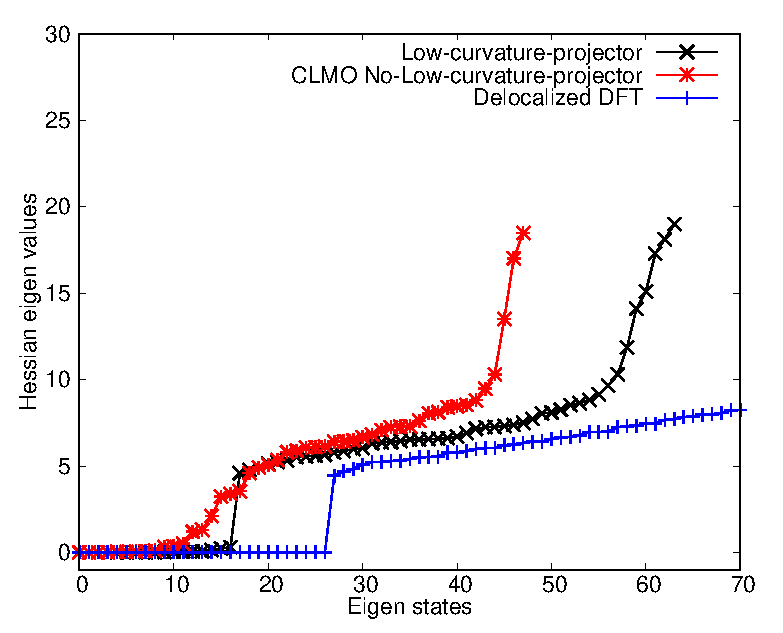
\includegraphics[width=0.4\textwidth]{Hesseig}
\caption{Eigenvalue spectra of Hessian during the optimization. The calculation is done on hexagonal CdSe lattice with 8 atoms. For the CLMO calculations the localization center is Cd$^{2+}$ ion and the domain includes one Cd$^{2+}$ and 3 Se$^{-2}$. For delocalized calculation the Hessian is for the complete system (only a portion of the eigenvalues are shown to save space). For the straight forward CLMO calculation without low-curvature-projector, the calculation won't converge and the Hessian is chosen at a stage where the energy is close to the ground state, for the other 2 cases the Hessian is chosen at convergence. PBE/DZVP level of theory is used for all cases.}
\label{sfig:hesseig}
\end{figure}

Here we give more details on our hypothesis in Eq.~\ref{eq:C}. The states $\ket{\psi_{yi}}$ are chosen so that: 
\bea
\braket{\psi_{yj}}{\psi_{yj}} - \bra{\psi_{yj}}\op{I_{x}}\ket{\psi_{yj}} < t
\eea

Fig~\ref{sfig:t_delta} shows that as $t$ increases and more states are chosen, $\Delta_{\bar{x}p}$ in Eq~\ref{eq:residue} gets smaller. The assumption is good for most weakly interacting materials but for Si where electrons are less localized the assumption is less accurate. Note however the validity of our method doesnot depend on this assumption.

\begin{figure}
\centering
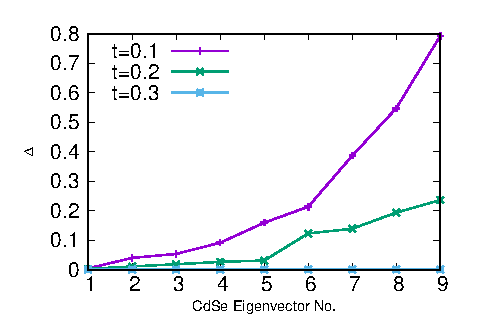
\includegraphics[width=0.3\textwidth]{t_cdse_residue}
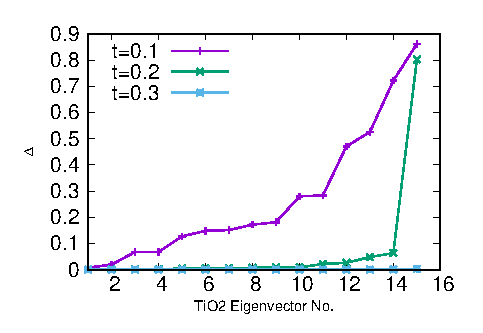
\includegraphics[width=0.3\textwidth]{t_tio2_residue}
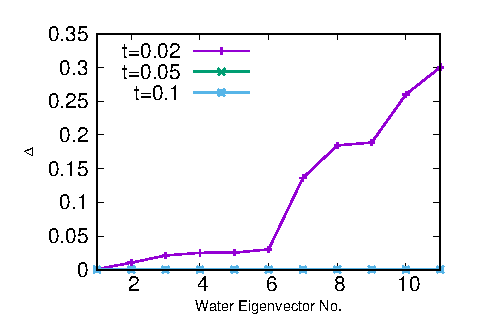
\includegraphics[width=0.3\textwidth]{t_water_residue}
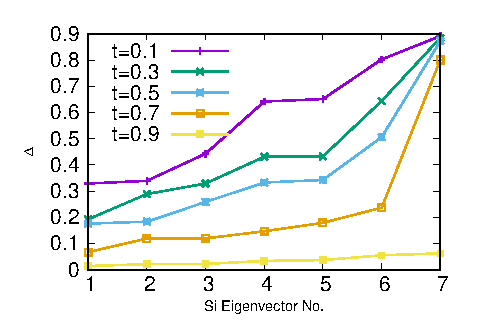
\includegraphics[width=0.3\textwidth]{t_si_residue}
\caption{$\Delta_{\bar{x}p}$ as a function of $t$, for materials studied in Fig~\ref{fig:projection}. As $t$ increases, $\Delta_{\bar{x}p}$ quickly reduces. Our assumption works well for most system except for Si.}
\label{sfig:t_delta}
\end{figure}
\end{document}
